\documentclass[10pt]{beamer}
\usepackage{graphicx}
\usepackage{amsmath,amssymb,amstext,xargs,ifthen}
\usepackage{amsfonts}
\usepackage{bbm,tikz}
\usepackage{beamerthemesplit}
\usetikzlibrary{arrows}

\usepackage[utf8]{inputenc}
\usepackage[french]{babel}

\usetheme{Antibes}
\mode<presentation>
\useoutertheme{tree}
\usecolortheme{beaver}
\useinnertheme{rectangles}

\setbeamerfont{block title}{size={}}
%\usecolortheme[rgb={0.55,0.1,0.05}]{structure}
%\usecolortheme[rgb={0.75,0.1,0.05}]{structure}
\usepackage{color}
\def\rset{\mathbb{R}}

\def\1{\mathbbm{1}}
\def\mcb{\ensuremath{\mathcal{B}}}
\def\mcc{\ensuremath{\mathcal{C}}}
\def\mce{\ensuremath{\mathcal{E}}}
\def\mcf{\ensuremath{\mathcal{F}}}
\def\nset{\ensuremath{\mathbb{N}}}
\def\qset{\ensuremath{\mathbb{Q}}}
\def\rset{\ensuremath{\mathbb{R}}}
\def\zset{\ensuremath{\mathbb{Z}}}
\def\cset{\ensuremath{\mathbb{C}}}
\def\rsetc{\ensuremath{\overline{\rset}}}
\def\Xset{\ensuremath{\mathsf{X}}}
\def\Tset{\ensuremath{\mathsf{T}}}
\def\Yset{\ensuremath{\mathsf{Y}}}
\def\rmd{\mathrm{d}}
\def\Qint{\ensuremath{\mathrm{QInt}}}
\def\Int{\ensuremath{\mathrm{Int}}}
\def\eqdef{\ensuremath{\stackrel{\mathrm{def}}{=}}}
\def\eqsp{\;}
\def\lleb{\lambda^{\mathrm{Leb}}}
\newcommand{\rmi}{\mathrm{i}}
\newcommand{\rme}{\mathrm{e}}
\def\supp{\mathrm{supp}}
\newcommand{\Cov}[2]{\mathrm{Cov}(#1,#2)}


%notation fourier
\def\1{\mathbbm{1}}
\def\mcb{\ensuremath{\mathcal{B}}}
\def\mcc{\ensuremath{\mathcal{C}}}
\def\mce{\ensuremath{\mathcal{E}}}
\def\mcf{\ensuremath{\mathcal{F}}}
\def\nset{\ensuremath{\mathbb{N}}}
\def\qset{\ensuremath{\mathbb{Q}}}
\def\rset{\ensuremath{\mathbb{R}}}
\def\cset{\ensuremath{\mathbb{C}}}
\def\rsetc{\ensuremath{\overline{\rset}}}
\def\Xset{\ensuremath{\mathsf{X}}}
\def\Tset{\ensuremath{\mathsf{T}}}
\def\Yset{\ensuremath{\mathsf{Y}}}
\def\rmd{\mathrm{d}}
\def\Qint{\ensuremath{\mathrm{QInt}}}
\def\Int{\ensuremath{\mathrm{Int}}}
\def\eqdef{\ensuremath{\stackrel{\mathrm{def}}{=}}}
\def\eqsp{\;}
\def\lleb{\lambda^{\mathrm{Leb}}}
\newcommand{\coint}[1]{\left[#1\right[}
\newcommand{\ocint}[1]{\left]#1\right]}
\newcommand{\ooint}[1]{\left]#1\right[}
\newcommand{\ccint}[1]{\left[#1\right]}

\def\bu{\mathbf{u}}
\newcommand{\TF}{\mathcal{F}}
\newcommand{\TFC}{\overline{\mathcal{F}}}
\newcommand{\TFA}[1]{\mathcal{F}\left( #1 \right)}
\newcommand{\TFAC}[1]{\overline{\mathcal{F}}\left( #1 \right)}

\def\TFyield{\stackrel{\mathcal{F}}{\mapsto}}

\def\tore{\mathbb{T}}
\def\btore{\mathcal{B}(\tore)}
\def\espaceproba{(\Omega,\mathcal{A},\PP)}
\def\limn{\lim_{n \rightarrow \infty}}
\newcommand{\ps}{\ensuremath{\text{p.s.}}}
\newcommand{\pp}{\ensuremath{\text{p.p.}}}
\def\cA{\mathcal{A}}
\def\cC{\mathcal{C}}
\def\cL{\mathcal{L}}
\def\cM{\mathcal{M}}
\def\cN{\mathcal{N}}
\def\cO{\mathcal{O}}
\def\cP{\mathcal{P}}
\def\cS{\mathcal{S}}
\newcommand{\filtop}[1]{\operatorname{F}_{#1}}
\def\bfphi{{\boldsymbol{\phi}}}
\def\bfpsi{{\boldsymbol{\psi}}}
\def\bfgamma{{\boldsymbol{\gamma}}}
\def\bfpi{{\boldsymbol{\pi}}}
\def\bfsigma{{\boldsymbol{\sigma}}}
\def\bftheta{{\boldsymbol{\theta}}}
\def\bfhphi{{\hat{\boldsymbol{\phi}}}}
\def\bfhrho{{\hat{\boldsymbol{\rho}}}}
\def\bfhgamma{{\hat{\boldsymbol{\gamma}}}}

\def\ltwo{L_2}
\newcommand{\lone}{\ensuremath{L_1}}

\newcommand{\pltwo}{\ensuremath{\ell^2}(\zset)}
\newcommand{\plone}{\ensuremath{\ell^1}(\zset)}
\newcommand{\plinfty}{\ensuremath{\ell^\infty}(\zset)}
\newcommand{\plp}{\ensuremath{\ell^p}(\zset)}

\def\calG{\mathcal{G}}
\def\calM{\mathcal{M}}
\def\calI{\mathcal{I}}
\def\calH{\mathcal{H}}


\newcommand\BL[1]{\mathrm{BL}(#1)}%bande limit{\'e}e
%Espace de Schwarz
\def\mcs{\ensuremath{\mathcal{S}}}
%produit scalaire
\newcommand{\pscal}[2]{\left\langle #1, #2 \right\rangle}
\newcommand{\proj}[3][]{
\ifthenelse{\equal{#1}{}}{\ensuremath{\operatorname{proj}\left( \left. #2\right|#3\right)}}
{\ensuremath{\operatorname{proj}_{#1}\left( \left. #2 \right|#3\right)}}
}
%espaces engendr{\'e}s
\newcommand{\lspan}[1]{\mathrm{Vect}(#1)}
\newcommand{\cspan}[1]{\overline{\mathrm{Vect}(#1)}}
\def\oplusperp{\stackrel{\perp}{\oplus}}
\def\ominusperp{\ominus}%\def\ominusperp{\stackrel{\perp}{\ominus}}


%Operation sur les fonctions/distributions

\newcommand{\translation}{\mathcal{T}}
\newcommand{\multiplication}{\mathcal{M}}


%
\def\Rset{\mathbb{R}}
\def\Cset{\mathbb{C}}
\def\Zset{\mathbb{Z}}
\def\Nset{\mathbb{N}}
\def\Tset{\mathrm{T}}
% et d'autres
\newcommand{\vvec}[1]{\mathbf{#1}}
\newcommand{\signe}{\mathrm{sgn}}
\newcommand{\rect}{\mathrm{rect}}
\newcommand{\sinc}{\mathrm{sinc}}
\newcommand{\cov}{\mathrm{cov}}
\newcommand{\corr}{\mathrm{corr}}
\newcommand{\vp}{\mathrm{vp}}
\newcommand{\erf}{\mathrm{erf}}
\def\cF{\mathcal{F}}
\def\cE{\mathcal{E}}
\def\cB{\mathcal{B}}
\def\cH{\mathcal{H}}
\def\cG{\mathcal{G}}
\def\cI{\mathcal{I}}
\def\PP{\mathbb{P}}
\newcommand\PE[1]{{\mathbb E}\left[ #1 \right]}
\newcommand{\Var}[1]{\mathrm{Var}\left( #1 \right)}
\def\BB{\mathrm{B.B.}}
\def\BBF{\mathrm{B.B.F.}}
\newcommandx{\norm}[2][2=]{\left\Vert #1 \right\Vert_{#2}}
\newcommandx{\opernorm}[2][2=]{{\left\vert\kern-0.25ex\left\vert\kern-0.25ex\left\vert #1
    \right\vert\kern-0.25ex\right\vert\kern-0.25ex\right\vert}_{#2}}
\def\L1loc{L_{1,\mathrm{loc}}}
\def\Leb{\mathrm{Leb}}


\newcommandx\sequence[3][2=,3=]
{\ifthenelse{\equal{#3}{}}{\ensuremath{\{ #1_{#2}\}}}{\ensuremath{\{ #1_{#2}, \eqsp #2 \in #3 \}}}}
\newcommandx\sequencePar[3][2=,3=]
{\ifthenelse{\equal{#3}{}}{\ensuremath{\{ #1({#2})\}}}{\ensuremath{\{ #1({#2}), \eqsp #2 \in #3 \}}}}
\def\pp{\ensuremath{\mathrm{p.p.}}}
\def\ie{i.e.}

\newcommand{\ensemble}[2]{\left\{#1\,:\eqsp #2\right\}}
\newcommand{\set}[2]{\ensemble{#1}{#2}}
\def\retard{\operatorname{S}}
\def\foo{\rme^{-2 \rmi \pi \nu}}
\def\cfoo{\rme^{+2 \rmi \pi \nu}}
\def\toref{\coint{-1/2,1/2}} 
\title{MAP 555 : Digital Filters...}
\begin{document}
\date{9 Octobre 2015}
\maketitle



\begin{frame}
\frametitle{Today}
\tableofcontents
\end{frame}

\section{Discrete-Time systems}
\begin{frame}
\frametitle{Discrete-time systems}
Denote by $\Xset$ and $\Yset$ the subspaces  of input and output signals satisfying the following assumptions:
\begin{enumerate}
\item $\Xset$ and $\Yset$ are  linear subspaces of the vector space  (over $\rset$ or $\cset$) of real or complex sequences indexed by $\zset$
\item $\Xset$ and $\Yset$ closed under translation: if $x \in \Xset$, then for any $a \in \zset$, $\retard_\tau x= \{ x[n-\tau], n \in \zset \} \in \Xset$, for all $\tau \in \zset$ and $x= \seqpar{x}[n][\zset] \in \Xset$ (and similarly for $\Yset$).
\end{enumerate}
\begin{definition}
A discrete-time system $T: \Xset \to \Yset$ is an operator that maps an input sequence $x= \seqpar{x}[n][\nset] \in \Xset$ into an output sequence $y= \seqpar{y}[n][\zset]$.
\alert{$$
y=T(x) \eqsp.
$$
}
\end{definition}
%\begin{itemize}
%\item The previous equation represents a rule or formula for computing the output sequence values from the input sequence values.
%\item It should be emphasized that the value of the output sequence at each value of the index $n$ may depend on $x[n]$ for all values of $n$.
%\item Systems are called \alert{memoryless} if $y[n]$ depends only on $x[n]$.
%\end{itemize}
\end{frame}

\begin{frame}
\frametitle{Examples}
\begin{itemize}
\item \alert{The ldeal Delay System}:
$$
y[n]=x[n-n_{d}],\ -\infty<n<\infty,
$$
where $n_{d}$ is a fixed positive integer called the delay of the system.
\item \alert{Moving averages} $\sum_{k=-\infty}^{\infty} |\psi_k| < \infty$, $\Xset= \plinfty$, $\Yset= \plinfty$
$$
y[n]= \sum_{k=-m}^p \psi_k x[n-k]
$$
\item \alert{Compressor} (or sub-sampling)
$$
y[n]= x[Mn] \eqsp, \quad n \in \zset
$$
\item \alert{Interpolator} (or up-sampling)
$$
y[n]= x[n/M] \quad \text{if $[n]_M= 0$ and $y[n]=0$ otherwise}
$$
\item \alert{Quadrator}
$$
y[n]= x^2[n] \eqsp, \quad n \in \zset \eqsp.
$$
\end{itemize}
\end{frame}

\begin{frame}
\frametitle{Linear Systems}
\begin{definition}[Linear Systems]
A system $T$ on a linear subspace $\Xset$ is linear if
$$
T( a_1 x_{1}+a_2 x_{2})=a_1 T(x_1) + a_2 T(x_2) \eqsp.
$$
\end{definition}
\begin{itemize}
\item A pure delay system is linear
\item The moving average is linear
\item The compressor and the interpolator are both linear
\item The quadrator is nonlinear!
\end{itemize}
\end{frame}

\begin{frame}
\frametitle{Time-invariance}
\begin{definition}[Time invariant]
A system $T$ on $\Xset \to \Yset$ is \alert{time-invariant}, if for all $\tau \in \zset$,
\alert{
$$
\retard_{\tau} \circ T = T \circ \retard_\tau
$$
}
\end{definition}
In words, a time-invariant system (often referred to equivalently as a shift-invariant system) is a system for which a time shift or delay of the input sequence causes a corresponding shift in the output sequence.
\begin{itemize}
\item The pure delay and the moving-average are linear and time-invariant.
\item The quadrator is time-invariant (but not linear)
\item The compressor and the interpolator are both linear but not time-invariant.
\end{itemize}
\end{frame}



\begin{frame}
\frametitle{Causality}
\begin{definition}[Causal or non-anticipative system]
A system is \alert{causal} or \alert{non-anticipative} if for any $n_0 \in \zset$ and $x_1, x_2 \in \Xset$ satisfying $x_1[n]= x_2[n]$, $n \leq n_0$, we have $y_1[n]= y_2[n]$ for $n \leq n_0$, where $y_1= T(x_1)$ and $y_2= T(x_2)$.
\end{definition}
\begin{itemize}
\item The pure delay is causal.
\item The moving average is causal if $\psi_k=0$ for any $k < 0$.
\item The quadrator is non-linear but causal (any memoryless transformation is causal)
\item The compressor and the interpolator are both causal
\end{itemize}
\end{frame}

\begin{frame}
\frametitle{Stability}
\begin{definition}[BIBO-Stability]
A system is stable in the bounded-input, bounded-output (BIBO) sense if and only if every bounded input sequence produces a bounded output sequence.
\end{definition}
\begin{itemize}
\item The pure delay is BIBO-stable.
\item The moving average is BIBO stable.
\item The quadrator is BIBO stable
\item The compressor and the interpolator are BIBO stable
\item $y[n]= \sum_{k=0}^n x[k]$ for $n \geq 0$ and $y[n]=0$ otherwise is linear, causal, but it is not BIBO-stable (it is not time invariant)
\end{itemize}

\end{frame}

\begin{frame}
\frametitle{Discrete convolution}
\begin{itemize}
\item Set $\Xset= \Yset= \plinfty$.
\item Let $\sequence{\psi}[k][\zset] \in \plone$. For any $x \in \plinfty$,
\[
\sup_{n \in \zset} |y[n]| \leq \sum_{k=-\infty}^\infty |\psi_k| \, \sup_{n \in \zset} |x[n]| \eqsp.
\]
\item For $x \in \Xset$, denote by $y = \psi * x$ the \alert{discrete convolution} of the sequences $\sequence{\psi}[k][\zset]$ and $\seqpar{x}[k][\zset]$:
\[
y[n]= \sum_{k=-\infty}^{\infty} \psi_k x[n-k]
\]
\item $y= T(x)= \psi * x$ is linear, time-invariant, BIBO stable. It is causal iff $\psi_k= 0$ for $k \leq 0$.
\item If $x= \delta$ the \alert{impulse sequence}, then $\psi= T(\delta)$: $\psi$ is the \alert{impulse response} of the system.
\end{itemize}
\end{frame}

\begin{frame}
\frametitle{LTI systems and convolutions}
\begin{itemize}
\item Let $T$ be a linear invariant system over $\Xset$. Assume that $\delta \in \Xset$ and denote by $\psi= T(\delta)$.
\item For any $x = \seqpar{x}[n][\zset]$ with \alert{finite support}, $x[n] = 0$ for $|n| \geq M$, we get
\[
x= \sum_{|k|\leq M} x[k] \tau_k \delta
\]
\item Hence,
\begin{align*}
y[n]&= T(x)[n]= \sum_{|k|\leq M} x[k] T(\tau_k \delta)[n] \\
&= \sum_{|k| \leq M} x[k] \tau_k T(\delta) [n]= \sum_{|k|\leq M} x[k] \psi_{n-k}
\end{align*}
\item Provided that the signal space is equipped with a norm and $T$ is continuous \wrt\ that norm, then it is possible to show that
every LTI systems can be represented as a \alert{linear convolution}.
\end{itemize}
\end{frame}
\subsection{Some properties of LTI systems}
\begin{frame}
\frametitle{Cascade connection}
\begin{itemize}
\item If $\sequence{\alpha}[k][\zset] \in \lone(\zset)$ and $\sequence{\beta}[k][\zset] \in \lone(\zset)$, then $\sum_{n = -\infty}^\infty \sum_{k= -\infty}^{\infty} |\alpha_k \beta_{n-k}| < \infty$ and $\alpha * \beta = \{( \alpha * \beta)_n, n \in \zset\}$ where
    \[
    (\alpha * \beta)_n = \sum_{k=-\infty}^{\infty} \alpha_k \beta_{n-k} \in \plone \eqsp.
    \]
In addition, $\alpha * \beta= \beta * \alpha$, the convolution on $\plone$ sequence is commutative.
\item For $\alpha \in \lone(\zset)$, define the LTI operator $\filter{\alpha}$ on $\plinfty$ by
\[
y= \filter{\alpha}(x)   \quad y[n]= \sum_{k \in \zset} \alpha_k x[n-k]
\]
\item If $\alpha \in \plone$ and $\beta \in \plone$, then
\alert{
\[
\filter{\alpha} \circ \filter{\beta} = \filter{\beta} \circ \filter{\alpha} = \filter{\alpha * \beta} = \filter{\beta * \alpha}\eqsp.
\]
}
\end{itemize}
\end{frame}

\section{The $z$-transform}
\subsection{Definition}
\begin{frame}
\frametitle{Why $z$-transform}
The $z$-transform is a generalization of discrete Fourier transform. Why generalize it?
\begin{itemize}
\item Fourier transform does not converge on all sequences. Hence the discussion of stability, causality, etc.. is blurred by convergence problems.
\item Bring the power of complex variable theory (poles, zeros, Laurent decomposition)
\end{itemize}
\end{frame}

\begin{frame}
\frametitle{Definition}
\begin{itemize}
\item The Fourier transform of a sequence $x \in \pltwo$ is defined as
\[
X(\rme^{\rmi \omega}) =_{\pltwo} \sum_{n=-\infty}^\infty x[n] \ec{n} \eqsp
\]
\item The $z$-transform of the sequence $x$ is defined as
\[
X(z)= \sum_{n=-\infty}^{\infty} x[n] z^{-n} \eqsp,
\]
which is, in general, an infinite sum or infinite power series, with $z$ being a complex variable.
\end{itemize}
\end{frame}



\begin{frame}
\frametitle{Bilateral z-transform}
\begin{itemize}
\item The $z$-transform can be seen as an operator which transforms the sequence $x$ into the function $X(z)$ , where $z$ is a continuous complex variable.
\item The correspondence between a sequence and its $z$-transform is indicated by the notation
$$
x[n] \ltz X(z)
$$
\item The $z$-transform $X(z)= \sum_{n=-\infty}^\infty x[n] z^{-n}$ is often referred to as the \alert{two-sided} or \alert{bilateral} $z$-transform, in contrast to the \alert{one-sided} or \alert{unilateral} $z$-transform, which is defined as
$$
X(z)\ =\sum_{n=0}^{\infty}x[n]z^{-n}
$$
\item Clearly, the bilateral and unilateral transforms are equivalent only if $x[n]=0$ for $n<0$.
\item In this lesson, we focus on the bilateral transform exclusively.
\end{itemize}
\end{frame}


\begin{frame}
\frametitle{$z$-transform and TFTD}
\begin{itemize}
\item It is evident  that there is a close relationship between the Fourier transform and the $z$-transform.
\item In particular, if we replace the complex variable $z$ in $X(z)= \sum_{n=-\infty}^{\infty} x[n] z^{-n}$ with the complex variable $\rme^{\rmi\omega}$, then the $z$-transform reduces to the DTFT.
\item This is one motivation for the notation $X(\rme^{\rmi \omega})$ for the Fourier transform; when it exists, the Fourier transform is simply $X(z)$ with $z=\rme^{\rmi \omega}$ which  corresponds to restricting $z$ to have unity magnitude; i.e., for $|z| =1$, the $z$-transform corresponds to the Fourier transform.
\end{itemize}
\end{frame}

\begin{frame}
\frametitle{Region of convergence}
\begin{itemize}
\item The $z$-transform does not converge for all sequences or for all values of $z$.
\item For any given sequence $x$, the set of values of $z$ for which the $z$-transform converges is called the \alert{region of convergence}, which we abbreviate \alert{$\ROC{x}$}.
\item Formally, $z \in \ROC{x}$ if
$$
\sum_{n=-\infty}^{\infty}|x[n]| |z|^{-n}<\infty
$$
\item For example, the sequence $x[n]=u[n]$ is not absolutely summable, and therefore, the Fourier transform does not converge absolutely. However, $\{ r^{-n}u[n], n \in \zset\}$ is absolutely summable if $r>1$. This means that the $z$-transform for the unit step exists with a region of convergence $|z|>1$.
\end{itemize}
\end{frame}

\begin{frame}
\frametitle{Region of convergence}
\begin{itemize}
\item If some value of $z$, say, $z=z_{1}$, is in the $\ROC{x}$, then all values of $z$ on the circle defined by $|z|=|z_{1}|$ will also be in the $\ROC{x}$.
\item  As one consequence of this, the region of convergence will consist of a ring in the $z$-plane centered about the origin.
\item  Its outer boundary will be a circle (or $\ROC{x}$ may extend outward to infinity), and its inner boundary will be a circle (or it may extend inward to include the origin).
\item If $\ROC{x}$ includes the unit circle, this of course implies convergence of the $z$-transform for $|z|=1$, or equivalently, the Fourier transform of the sequence converges.
\item Conversely, if the $\ROC{x}$ does not include the unit circle, the Fourier transform does not converge absolutely.
\end{itemize}
\end{frame}


\begin{frame}
\frametitle{The $z$-transform is not always defined}
\begin{itemize}
\item Uniform convergence of the $z$-transform requires absolute summability of the exponentially weighted sequence.
\item Neither of the sequences
\begin{align*}
x_{1}[n] &=\frac{\sin\omega_{c}n}{\pi n}, && n \in \zset \\
x_{2}[n] &=\cos\omega_{0}n,&& n \in \zset
\end{align*}
is absolutely summable. Furthermore, neither of these sequences multiplied by $r^{-n}$ would be absolutely summable for any value of $r$.
\item Thus, these sequences do not have a $z$-transform that converges absolutely for any $z$.
\item However,  even though sequences such as $x_{1}[n]$ is not absolutely summable, $x_1 \in \pltwo$, and the Fourier transform converges in the mean-square sense to a discontinuous periodic function.
\end{itemize}
\end{frame}

\begin{frame}
\frametitle{Rational models}
\begin{itemize}
\item Among the most important and useful $z$-transforms are those for which $X(z)$ is a rational function inside the region of convergence, i.e.,
$$
X(z)=\frac{P(z)}{Q(z)}
$$
where $P(z)$ and $Q(z)$ are polynomials in $z$.
\item The values of $z$ for which $X(z)=0$ are called the \alert{zeros} of $X(z)$ , and the values of $z$ for which $X(z)$ is infinite are referred to as the \alert{poles} of $X(z)$ .
\item The poles of $X(z)$ for finite values of $z$ are the roots of the denominator polynomial. In addition, poles may occur at $z=0$ or $ z=\infty$.
\item For rational $z$-transforms, a number of important relationships exist between the locations of poles of $X(z)$ and the region of convergence of the $z$-transform. (\alert{wait...})
\end{itemize}
\end{frame}


\begin{frame}
\frametitle{Right-sided exponential sequence}
\begin{itemize}
\item Consider the signal $x[n]=a^{n}u[n]$. Because it is nonzero only for $n\geq 0$, this is an example of a \alert{right-sided} sequence.
$$
X(z)=\sum_{n=-\infty}^{\infty} a^{n}u[n]z^{-n}=\sum_{n=0}^{\infty}(az^{-1})^{n}
$$
\item For convergence of $X(z)$ , we require that
$$
\sum_{n=0}^{\infty}|az^{-1}|^{n}<\infty.
$$
Thus, the region of convergence is the range of values of $z$ for which $|az^{-1}|<1$ or, equivalently, $|z|>|a|$.
\item Inside the region of convergence, the infinite series converges to
$$
X(z)\ =\sum_{n=0}^{\infty}(az^{-1})^{n}=\frac{1}{1-az^{-1}}=\frac{z}{z-a},\ |z|>|a|.
$$
\end{itemize}
\end{frame}

\begin{frame}
\frametitle{Right-sided exponential sequence}
\begin{itemize}
\item The $z$-transform has a region of convergence for any finite value of $|a|$. The Fourier transform of $x[n]$, on the other hand, converges only if $|a|<1$.

\item The infinite sum is equal to a rational function of $z$ inside the region of convergence; for most purposes, this rational function is a much more convenient representation than the infinite sum.
\item We will see that any sequence that can be represented as a sum of exponentials can equivalently be represented by a rational $z$-transform.
\item Such a $z$-transform is determined to within a constant multiplier by its \alert{zeros} and its \alert{poles}.
\end{itemize}
\end{frame}



\begin{frame}
\frametitle{Right-sided exponential sequence}
\begin{figure}
  \centering
  % Requires \usepackage{graphicx}
  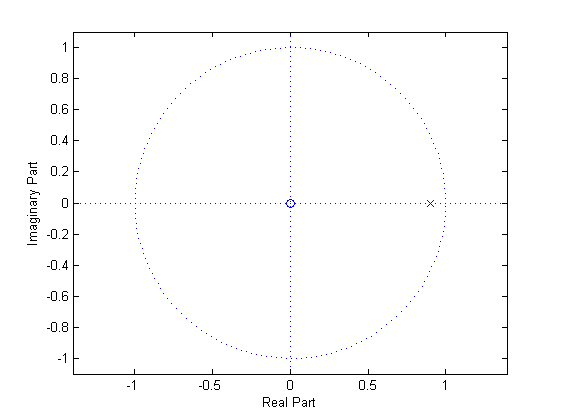
\includegraphics[width=0.6\textwidth]{polezeroonesided.png}\\
  \caption{For right-sided exponential sequence, there is one zero, at $z=0$, and one pole, at $z=a$.}
\end{figure}
\end{frame}

\begin{frame}
\frametitle{Left-sided exponential sequence}
\begin{itemize}
\item Now let $x[n]=-a^{n}u[-n-1]$. Since the sequence is nonzero only for $n\leq-1$, this is a \alert{left-sided} sequence.
Then
\begin{align*}
X(z)&=-\sum_{n=-\infty}^{\infty}a^{n}u[-n-1]z^{-n}=-\sum_{n=-\infty}^{-1}a^{n}z^{-n} \\
&=-\sum_{n=1}^{\infty}a^{-n}z^{n}=1-\sum_{n=0}^{\infty}(a^{-1}z)^{n}
\end{align*}
\item If $|a^{-1}z|<1$ or, equivalently, $|z|<|a|$, the sum  converges, and
$$
X(z)=1-\frac{1}{1-a^{-1}z}=\frac{1}{1-az^{-1}}=\frac{z}{z-a},\ |z|<|a|.
$$
\end{itemize}
\end{frame}

\begin{frame}
\frametitle{Always specify the ROC !}
\begin{itemize}
\item We see that the right-sided and left-sided exponential sequences are different and, therefore, the infinite sums are different;
\item however, the algebraic expressions for $X(z)$ and the corresponding pole-zero plots are identical !
\item The $z$-transforms differ only in the \alert{region of convergence}.
\item This emphasizes the need for specifying \alert{both} the \alert{algebraic expression} and \alert{the region of convergence} for the $z$-transform of a given sequence.
\end{itemize}
\end{frame}


\begin{frame}
\frametitle{Some common $z$-transform}
\begin{tabular}{lll}
1. $\delta[n]$ &1 &  $\cset$ \\
2. $u[n]$ &  $\frac{1}{1-z^{-1}}$& $|z|>1$ \\
3. $-u[-n-1]$ & $\frac{1}{1-z^{-1}}$& $|z|<1$ \\
4. $\delta[n-m]$& $ z^{-m}$ &  $\cset \setminus \{0\}$ if $m>0$\\
               &           & or $\cset \setminus \infty$ if $m < 0$\\
5. $a^{n}u[n]$ & $\frac{1}{1-az^{-1}}$ & $|z|>|a|$ \\
6. $-a^{n}u[-n-1]$ & $\frac{1}{1-az^{-1}}$ & $|z|<|a|$ \\
7. $na^{n}u[n]$ & $\frac{az^{-1}}{(1-az^{-1})^{2}}$  & $|z|>|a|$ \\
8. $-na^{n}u[-n-1]$ & $\frac{az^{-1}}{(1-az^{-1})^{2}}$ & $|z|<|a|$ \\
9. $[\cos\omega_0n]u[n]$& $\frac{1-[\cos\omega_0]z^{-1}}{1-[2\cos\omega_0]z^{-1}+z^{-2}}$ & $|z|>1$\\
10. $[\sin\omega_0n]u[n]$& $\frac{[\sin\omega_{0}]z^{-1}}{1-[2\cos\omega_0]z^{-1}+z^{-2}}$ & $|z|>1$\\
11. $[r^{n}\cos\omega_0 n]u[n]$ &$\frac{1-[r\cos\omega_0]z^{-1}}{1-[2r\cos\omega_0]z^{-1}+r^{2} z^{-2}}$ &$ |z|>r$ \\
12. $[r^{n}\sin\omega_0n]u[n]$ & $\frac{[r\sin\omega_0]z^{-1}}{1-[2r\cos\omega_0]z^{-1}+r^{2}z^{-2}}$ &$|z|>r$
\end{tabular}
\end{frame}

\begin{frame}
\frametitle{Properties of the $z$-transform}
\begin{itemize}
\item \alert{Property 1}: The ROC is a ring or disk in the $z$-plane centered at the origin; i.e.,
$$
 0\leq r_{R}<|z|<r_{L}\leq\infty.
$$
\item \alert{Property 2}: The Fourier transform of $x[n]$ converges absolutely if and only if the ROC of the $z$-transform of $x[n]$ includes the unit circle.
\item \alert{Property 3}: The ROC cannot contain any poles.
\item \alert{Property 4}: If $x[n]$ is a \alert{finite-duration sequence}, then the ROC is the entire $z$-plane, except possibly $z=0$ or $ z=\infty$.
\end{itemize}
\end{frame}

\begin{frame}
\frametitle{Properties of the $z$-transform}
\begin{itemize}
\item \alert{Property 5}: If $x[n]$ is a \alert{right-sided sequence}, i.e., a sequence that is zero for $ n<N_{1}<\infty$, the ROC extends outward from the \alert{outermost} (i.e., largest magnitude) finite pole in $X(z)$ to (and possibly including) $ z=\infty$.
\item \alert{Property 6}: If $x[n]$ is a \alert{left-sided sequence}, i.e.. a sequence that is zero for $n>  N_{2}>-\infty$, the ROC extends inward from the \alert{innermost} (smallest magnitude) nonzero pole in $X(z)$ to (and possibly including) $z=0$.
\item \alert{Property 7}: A \alert{two-sided sequence} is an infinite-duration sequence that is neither right sided nor left sided. if $x[n]$ is a two-sided sequence, the ROC will consist of a ring in the $z$-plane, bounded on the interior and exterior by a pole and, consistent with property 3, not containing any poles.
\item \alert{Property 8}: The ROC must be a connected region.
\end{itemize}
\end{frame}
\subsection{Inverse $z$-transform}
\begin{frame}
\frametitle{Laurent Decomposition}
\begin{itemize}
\item If a function is analytic over an annular domain $r < |z| < R$, then the Laurent series expansion
shows that $X(z)$ can be decomposed as
\[
X(z)= \sum_{n=-\infty}^\infty a_n z^{-n} \quad a_n= \frac{1}{2 \pi \rmi} \int_{\gamma} X(z) z^{n-1} \rmd \xi
\]
where $\gamma$ is any rectifiable path containing no self-intersections in the annulus.
\item The series is absolutely converging in any compact domain of the $\{r < |z| < R\}$
\end{itemize}
\end{frame}



\begin{frame}
\frametitle{Laurent series}
\begin{itemize}
\item A Laurent series (therefore the $z$-transform) is analytic over $0 \leq r < |z| < R \leq \infty$; hence, the $z$-transform and all its derivatives must be infinitely differentiable functions of $z$ within the region of convergence.
\item This implies that if the region of convergence includes the unit circle, then the Fourier transform and all its derivatives with respect to $\omega$ must be continuous functions of $\omega$.
\item Also,  the sequence must be absolutely summable, i.e., a stable sequence.
\end{itemize}
\end{frame}

\begin{frame}
\frametitle{Inverse $z$-transform}
\begin{itemize}
\item Beware !...  Always specify the ROC on which you are willing to invert... there are has many possible inverse than the number of possible ROCs!
\item When $X(z)= P(z)/Q(z)$ is a rational the easiest way to proceed is to use \alert{partial fraction expansion}. Assuming that $\deg P < \deg Q=N$, assuming simple poles write
\[
X(z)= \sum_{k=1}^N \frac{A_k}{1-p_k z^{-1}}
\]
where $N= \deg Q$ and $p_1,\dots,p_N$ are the \alert{poles} (the zeros of $Q(z)$) and $A_k= \lim_{z \to p_k} (z-p_k) X(z)$ is the
\alert{residue} at pole $p_k$. We assume that $|p_1| < |p_2| < \dots <|p_N|$
\item Assume first that we are willing to invert the $z$-transform on $|z| > R$, where $R > \max_{1 \leq k \leq N}( |p_k|)$. Then
\[
x[n] = \sum_{k=1}^N p_k^n u[n]
\]
\end{itemize}
\end{frame}

\begin{frame}
\frametitle{Inverse $z$-transform}
\begin{itemize}
\item Assume now that we are inverting on  $|p_{\ell}| < |z| < |p_{\ell+1}|$ for some $\ell \in \{1, \dots, N-1\}$.
We need to consider the two possible expansions for each factor in the decomposition
\begin{align*}
&\frac{1}{1-p_k z^{-1}} = \sum_{n=0}^\infty p_k^{n} z^{-n} && |p_k| < |z| \quad \text{\alert{causal}} \\
&\frac{1}{1-p_k z^{-1}} = - \sum_{n=-\infty}^{-1} p_k^n z^{-n} && |p_k| > |z| \quad \text{\alert{anti-causal}} \text\eqsp.
\end{align*}
\item Hence, the inverse $z$-transform is
\[
x[n] = \sum_{k=1}^\ell p_k^n u[n] - \sum_{k=\ell+1}^N p_k^n u[-n-1]
\]
\end{itemize}
\end{frame}


\begin{frame}
\frametitle{Other techniques: power series expansion}
The function $X(z)= \log(1 + a z^{-1})$  is analytic for $|z| > |a|$. A power series expansion show that, converging on the $|z| > |a|$ shows that
\[
\log(1 + az ^{-1}) = \sum_{n=1}^\infty (-1)^{n+1} \frac{a^n}{n} z^{-n} \eqsp, \quad |z| > |a|
\]
showing that
\[
x[n]= (-1)^{n+1} \frac{a^n}{n} u[n-1]
\]

\end{frame}

\begin{frame}
\frametitle{Inverse $z$-transform: contour integration}
\begin{itemize}
\item If $X(z)$ is analytic on $0 \leq r < |z| < R \leq \infty$, then for any   closed rectifiable curve $\gamma$ inside the ROC and any $n \in \nset$
\[
x[n]= \frac{1}{2 \pi \rmi} \oint_{\gamma} X(z) z^{n-1} \rmd z
\]
\item  \alert{Any contour give the same integral}
\item Best to use with the Cauchy residue theorem.
\end{itemize}
\end{frame}


\begin{frame}
\frametitle{Residue theorem}
Suppose $U$ is a simply connected open subset of the complex plane, and $a_1,\dots,a_n$ are finitely many points of $U$ and $f$ is a function which is defined and holomorphic on $U \setminus \{a_1,\dots,a_n\}$. If $\gamma$ is a closed rectifiable curve in $U$ which does not meet any of the $a_k$,
then
\[
\oint_\gamma f(z)\, \rmd z =
2\pi \rmi \sum_{k=1}^n \operatorname{I}(\gamma, a_k) \operatorname{Res}( f, a_k ).
\]
If $\gamma$ is a positively oriented simple closed curve, $I(\gamma, a_k) = 1$ if $a_k$ is in the interior of $\gamma$, and $0$ if not, so
\[
\oint_\gamma f(z)\, \rmd z =
2 \pi \rmi \sum \operatorname{Res}( f, a_k )
\]
with the sum over those $k$ for which $a_k$ is inside $\gamma$.
\end{frame}

\begin{frame}
\frametitle{Residue theorem}
At a simple pole $c$, the residue of $f$ is given by:
$$
\operatorname{Res}(f,c)=\lim_{z\to c}(z-c)f(z).
$$
More generally, if $c$ is a pole of order $n$, then the residue of $f$ around $z = c$ can be found by the formula:
$$
 \mathrm{Res}(f,c) = \frac{1}{(n-1)!} \lim_{z \to c} \frac{d^{n-1}}{dz^{n-1}}\left( (z-c)^{n}f(z) \right).
$$ 
\end{frame}




\subsection{Property of the $z$-transform}
\begin{frame}
\frametitle{Linearity}
\begin{align*}
&y[n]= a_1 x_{1}[n]+ a_2 x_{2}[n]  \ltz a_1 X_{1}(z)+a_2 X_{2}(z) \eqsp,\\
&\ROC{y} \supset \ROC{x_{1}} \cap \ROC{x_2} \eqsp.
\end{align*}
\begin{itemize}
\item For sequences with rational $z$-transforms, if the poles of $a_1X_{1}(z)+a_2X_{2}(z)$ consist of all the poles of $X_{1}(z)$ and $X_{2}(z)$ (i.e., if there is no pole-zero cancellation), then the region of convergence will be exactly equal to the overlap of the individual regions of convergence.
\item If the linear combination is such that some zeros are introduced that cancel poles, then the region of convergence may be larger.
\end{itemize}
\end{frame}

\begin{frame}
\frametitle{Time-shifting and Differentiation}
\begin{align*}
&x[n-n_{0}] \ltz z^{-n_{0}}X(z) \quad \ROC{\retard_{n_0} x}= \ROC{x}
\end{align*}
(except for the possible addition or deletion of $z=0$ or $ z=\infty$).

\bigskip

The ROC can be changed, since the factor $z^{-n_{0}}$ can alter the number of poles at $z=0$ or $ z=\infty$.
$$
y[n]= n x[n] \ltz - z \frac{\rmd X(z)}{\rmd z} \eqsp, \quad \ROC{y}= \ROC{x} \eqsp.
$$
\end{frame}

\begin{frame}
\frametitle{Convolution of sequences}
$$
y[n]= x_1 * x_2[n] \ltz X_1(z) X_2(z) \eqsp, \ROC{y} \supset \ROC{x_1} \cap \ROC{x_2} \eqsp.
$$
\begin{itemize}
\item If $\ROC{x_1} \cap \ROC{x_2} = \emptyset$, then the convolution on the RHS is not defined.
\item  the convolution property plays a particularly important role in the analysis of LTI systems.
\item Specifically, as a consequence of this property, the $z$-transform of the \alert{output} of an LTI system is the \alert{product} of the $z$-transform of the \alert{input} and the $z$-transform of the \alert{system impulse response} called the \alert{transfer function}.
\end{itemize}
\end{frame}

\begin{frame}
\frametitle{Evaluating a convolution with the $z$-transform}
Let $x_{1}[n]=a^{n}u[n]$ and $x_{2}[n]=u[n]$. The corresponding $z$-transforms are
$$
X_{1}(z)=\sum_{n=0}^{\infty}a^{n}z^{-n}=\frac{1}{1-az^{-1}},\ |z|>|a|,
$$
and
$$
X_{2}(z)=\sum_{n=0}^{\infty}z^{-n}=\frac{1}{1-z^{-1}},\ |z|>1.
$$
If $|a|<1$, the $z$-transform of the convolution of $x_{1}[n]$ with $x_{2[n]}$ is then
$$
Y(z)=\frac{1}{(1-az^{-1})(1-z^{-1})}=\frac{z^{2}}{(z-a)(z-1)},\ |z|>1.
$$
The sequence $y[n]$ can be obtained by determining the inverse $z$-transform. Expanding $Y(z)$ on $|z|> 1$ in a partial fraction expansion, we get
$$
Y(z)=\frac{1}{1-a} \left\{ \frac{1}{1-z^{-1}}-\frac{a}{1-az^{-1}} \right\} \eqsp, \quad |z|>1,
$$
showing that
$$
y[n]=\frac{1}{1-a}(u[n]-a^{n+1}u[n])\ .
$$
\end{frame}


\section{Linear constant-coefficient difference equations}
\begin{frame}
\frametitle{constant-coefficient difference equation}
\begin{itemize}
\item Consider the class of systems whose input and output satisfy a linear constant-coefficient difference equation of the form
\alert{
$$
\sum_{k=0}^{N}a_{k}y[n-k]=\sum_{k=0}^{M}b_{k}x[n-k].
$$
}
\item Applying the $z$-transform to both sides  and using the \alert{linearity property} and the \alert{time-shifting} property,
we obtain
$$
\sum_{k=0}^{N}a_{k}z^{-k}\mathrm{Y}(z)=\sum_{k=0}^{M}b_{k}z^{-k}X(z)\ ,
$$
or equivalently,
$$
\left(\sum_{k=0}^{N}a_{k}z^{-k} \right) Y(z)= \left(\sum_{k=0}^{M}b_{k}z^{-k} \right) X(z) \eqsp.
$$
\end{itemize}
\end{frame}

\begin{frame}
\frametitle{System function}
\begin{itemize}
\item The system function has the algebraic form
$$
H(z)=\frac{Y(z)}{X(z)}=\frac{\sum_{k=0}^{M}b_{k}z^{-k}}{\sum_{k=0}^{N}a_{k}z^{-k}}
$$
\item $H(z)$  is a ratio of polynomials in $z^{-1}$, It is often convenient to express $H(z)$ in factored form as
$$
H(z)=\left(\frac{b_{0}}{a_{0}} \right)\frac{\prod_{k=1}^M (1-c_{k}z^{-1})}{\prod_{k=1}^{N}(1-d_{k}z^{-1})} \eqsp.
$$
\item Each of the factors $(1-c_{k}z^{-1})$ in the numerator contributes a zero at $z=c_{k}$ and a pole at $z=0$.
\item Similarly, each of the factors $(1-d_{k}z^{-1})$ in the denominator contributes a zero at $z=0$ and a pole at $z=d_{k}$.
\end{itemize}
\end{frame}

\begin{frame}
\frametitle{Stability and Causality}
\begin{itemize}
\item To transform the difference equation
$$
 \sum_{k=0}^{N}a_{k}y[n-k]=\sum_{k=0}^{M}b_{k}x[n-k] \quad \text{into} \quad Y(z)= \frac{B(z)}{A(z)} X(z) = H(z) X(z)
$$
we made no further assumption about stability or causality.
\item Correspondingly, from the difference equation, we can obtain the algebraic expression for the system function, but not the region of convergence. The region of convergence of $H(z)$ is \alert{not determined} from the derivation leading , since all that is required for $Y(z)= H(z) X(z)$ is that $X(z)$ and $Y(z)$ have overlapping regions of convergence !
\item \alert{Warning !}  \alert{the difference equation does not uniquely specify the impulse response of a linear time-invariant system} !
\end{itemize}
\end{frame}


\begin{frame}
\frametitle{Stability and Causality}
\begin{itemize}
\item For the system function $H(z)= B(z)/A(z)$, there are a number of choices for the region of convergence.
\item For a given ratio of polynomials, \alert{each possible choice for the region of convergence will lead to a different impulse response}, but they will all \alert{correspond to the same difference equation}.
\item However, \alert{if we assume that the system is causal}, it follows that $h[n]$ must be a right-sided sequence, and therefore, the region of convergence of $H(z)$ must be outside the outermost pole.
\item Alternatively, if we assume that \alert{the system is stable}, then,  the impulse response must be absolutely summable, i.e.,
$$
\sum_{n=-\infty}^{\infty}|h[n]|<\infty.
$$
\end{itemize}
\end{frame}

\begin{frame}
\frametitle{Determining the ROC}
\begin{itemize}
\item Consider the LTI system with input and output related through the difference equation
$$
y[n]-\frac{5}{2}y[n-1]+y[n-2]=x[n].
$$
\item The system function $H(z)$ is given by
$$
H(z)=\frac{1}{1-\frac{5}{2}z^{-1}+z^{-2}}=\frac{1}{(1-\frac{1}{2}z^{-1})(1-2z^{-1})}.
$$
\item The system has a zero (of order 2) at $0$ and two poles at $1/2$ and $2$. There are three possible choices for the ROC.
\begin{enumerate}
\item  If the system is assumed to be causal, then the ROC is outside the outermost pole, i.e., $|z|>2$. In this case the system will not be stable, since the ROC does not include the unit circle.
\item If we assume that the system is stable, then the ROC will be $1/2<|z| <2$. The system will not be causal.
\item For the third possible choice of ROC, $|z|< 1/2$, the system will be neither stable nor causal.
\end{enumerate}
\end{itemize}
\end{frame}

\begin{frame}
\frametitle{Stable and causal LTI}
\begin{itemize}
\item Causality and stability are not necessarily compatible requirements.
\item In order for a linear time-invariant system whose input and output satisfy a difference equation to be both causal and stable, the ROC of the corresponding system function \alert{must be outside the outermost pole}  and \alert{include the unit circle}. Clearly, this requires that all the poles of the system function be inside the unit circle.
\end{itemize}
\end{frame}

\begin{frame}
\frametitle{A first order IIR filter}
\begin{itemize}
\item Consider a  system whose input and output satisfy the difference equation
$$
y[n]-ay[n-1]\ =x[n]
$$
\item The system function is
$$
H(z)=\frac{1}{1-az^{-1}}.
$$
and has a \alert{single pole} at $a$.
\item There are two possible ROC $|z| > |a|$ and $|z| < |a|$.
\begin{enumerate}
\item If the system is assumed to be \alert{causal}, then the ROC should be outside the outermost pole  $|z|>|a|$.
\item if the system is assumed to be \alert{stable}, the unit circle should be included in $|z| > |a|$, which implies that $|a|<1$.
\end{enumerate}
\item For a \alert{causal} and \alert{stable} solution ($|a| < 1$), the associated impulse response is
$$
h[n]=a^{n}u[n]
$$
The impulse response has infinitely many no zero terms; this is an IIR LTI system.
\end{itemize}
\end{frame}

\begin{frame}
\frametitle{Frequency response for rational filters}
If a stable linear time-invariant system has a rational system function (i.e., if its input and output satisfy a difference equation), then its frequency response (the system function evaluated on the unit circle) has the form
$$
H(\rme^{\rmi\omega})=\frac{\sum_{k=0}^M b_k \rme^{-\rmi \omega k}}{\sum_{k=0}^N a_k \rme^{-\rmi \omega k}}
$$
That is, $H(\rme^{\rmi\omega})$ is a ratio of polynomials in the variable $\rme^{-\rmi\omega}$.
\end{frame}



\end{document} 